\chapter{长弦与黑洞对应}

\lectureoverview{黑洞具有熵，因此它必定拥有微观自由度。我们将建立关于这些自由度的最简单的弦论描述：首先对一条长激发弦的态进行计数，然后改变弦耦合，直到弦的描述与黑洞的描述相遇。最后的等式被有意留作下一讲要完成的问题。}

\section{熵要求微观载体}

说一个系统具有很大的熵，就是说它能够隐藏大量的微观信息。一浴缸热水可能具有量级为\(10^{30}\)的熵。这一陈述已经告诉我们，存在着数量极其巨大的微观自由度，无论我们是否选择逐个分子地去检视它们。热力学可以通过测量能量和温度来确定熵，但它并不指认携带熵的对象。

流体动力学使这一区分变得熟悉。它描述密度、速度、压强和宏观流动，而不提及原子。加上热力学，人们就会发现流体具有熵。熵宣告了一种粗粒化方程并不显示的微观结构；它引出一个新问题，而不是回答它。

黑洞以更尖锐的形式提出了同样的挑战。Bekenstein的提议，经Hawking的计算而完成，赋予熵一个与视界面积成正比的量。广义相对论确定了几何及其热力学，但它没有给出微观态的清单。那些其组态解释了面积律的微小而众多的对象是什么？在弦理论中存在一个具体的候选者。这里展开的论证是有意定性的：它把参数依赖关系弄对了，同时略去了数值常数和完整态计数的形式化机器。

\section{三个尺度与一个记号上的危险}

引力提供了一个特殊的长度，即普朗克长度，
\begin{equation}
\ell_p=\sqrt{\frac{G_N\hbar}{c^3}}.
\label{eq:l06-planck-si}
\end{equation}

\begin{classroomqa}
\audiencequestion{\(G_N\)、\(\hbar\)和\(c\)的哪种组合给出普朗克长度？\lecturetimestamp{00:06:08}}
\lecturerresponse{是\(\sqrt{G_N\hbar/c^3}\)，约为\(10^{-33}\)厘米。我们将立即令\(\hbar=c=1\)，于是该关系变得简单得多。}
\end{classroomqa}

在自然单位下，
\begin{equation}
\hbar=c=1,
\qquad
G_N=\ell_p^2.
\label{eq:l06-planck-area}
\end{equation}
因此牛顿常数具有面积的量纲。这就是为什么一个面积除以\(G_N\)是无量纲的，并且可以是一个熵。

弦理论有第二个长度，\(\ell_s\)。加热一条弦，或把它置于高度激发的态，它就会在许多尺度上摆动。在这一基本图像中，特征性的最短尺度是弦长。人们可以把\(\ell_s\)视为与弦振荡的一个基本单元相关联的尺度。

第三个量是无量纲的弦耦合\(g_s\)。它控制分裂与合并：一条弦可以掐断成两条弦，或者一条激发弦可以发射一个闭弦量子。

\begin{classroomqa}
\audiencequestion{弦耦合的物理意义是什么？\lecturetimestamp{00:09:20}}
\lecturerresponse{它控制弦发生相互作用的几率，例如当一条弦与自身相交时的分裂。更确切地说，\(g_s\)是相互作用振幅；相应的概率或速率从\(g_s^2\)阶开始。}
\end{classroomqa}

所发射的无质量闭弦激发可以是一个引力子。在这方面，\(g_s\)扮演着类似于电荷的角色：它是附着在一个相互作用顶点上的因子。\editorialnote{本讲在把\(g_s\)称为概率和称为振幅之间交替。在微扰论中，它是振幅层面的耦合；概率和速率则包含它的平方。}

\section{为什么引力知道\texorpdfstring{\(g_s^2\)}{耦合的平方}}

首先考虑电磁学的交换图像。一个带电物体发射一个光子，带有一个\(e\)因子，第二个物体吸收它，又带有一个\(e\)因子。因此交换振幅包含\(e^2\)。这一图像并不是字面意义上的经典抛射物故事，但它正确地显示了耦合如何进入。

\begin{figure}[htbp]
\centering
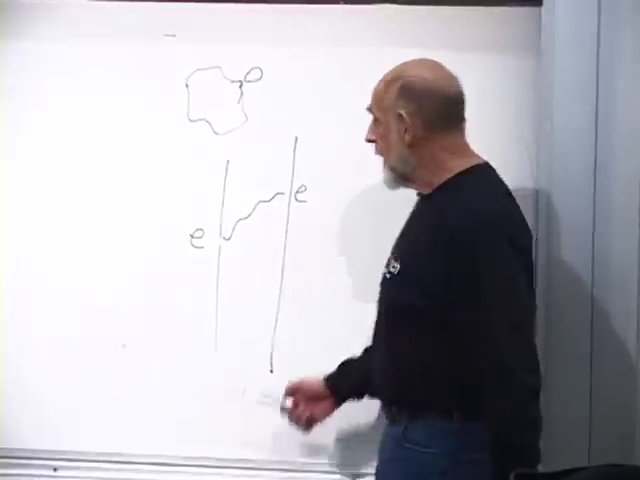
\includegraphics[width=0.72\textwidth]{lecture_06_figure_03.png}
\caption{黑板上完成的交换草图：一个耦合附着在发射处，又附着在吸收处。}
\lectureframe{00:11:30.000}
\end{figure}

弦理论的版本把光子替换为引力子，把电荷替换为\(g_s\)。一个因子伴随发射，另一个伴随吸收，因此引力强度按\(g_s^2\)标度。

在长距离下，同一相互作用必须重现牛顿的力定律，
\begin{equation}
F_{\mathrm{grav}}\sim G_N\frac{M_1M_2}{r^2}.
\end{equation}
质量和平方反比依赖关系描述源和传播；这里所需的要点是乘在它们前面的耦合。

\begin{figure}[htbp]
\centering
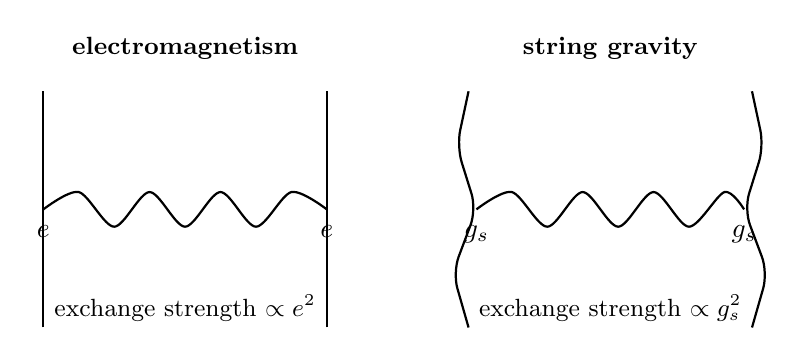
\begin{tikzpicture}[x=1cm,y=1cm]
  \node[font=\small\bfseries] at (1.8,3.55) {electromagnetism};
  \draw[line width=0.8pt] (0,0) -- (0,3);
  \draw[line width=0.8pt] (3.6,0) -- (3.6,3);
  \draw[line width=0.8pt] plot[smooth] coordinates {(0,1.5) (0.45,1.72) (0.9,1.28) (1.35,1.72) (1.8,1.28) (2.25,1.72) (2.7,1.28) (3.15,1.72) (3.6,1.5)};
  \node[below] at (0,1.42) {\(e\)};
  \node[below] at (3.6,1.42) {\(e\)};
  \node[font=\small] at (1.8,0.25) {exchange strength \(\propto e^2\)};
  \node[font=\small\bfseries] at (7.2,3.55) {string gravity};
  \draw[line width=0.8pt,rounded corners=6pt] (5.4,0) -- (5.2,0.7) -- (5.5,1.5) -- (5.25,2.3) -- (5.4,3);
  \draw[line width=0.8pt,rounded corners=6pt] (9,0) -- (9.2,0.7) -- (8.9,1.5) -- (9.15,2.3) -- (9,3);
  \draw[line width=0.8pt] plot[smooth] coordinates {(5.5,1.5) (5.95,1.72) (6.4,1.28) (6.85,1.72) (7.3,1.28) (7.75,1.72) (8.2,1.28) (8.65,1.72) (8.9,1.5)};
  \node[below] at (5.5,1.42) {\(g_s\)};
  \node[below] at (8.9,1.42) {\(g_s\)};
  \node[font=\small] at (7.2,0.25) {exchange strength \(\propto g_s^2\)};
\end{tikzpicture}
\caption{耦合计数类比。交换的量子每一端贡献一个相互作用因子。}
\end{figure}

这一观察几乎确定了牛顿常数。耦合\(g_s\)是无量纲的，而在四维中\(G_N\)具有长度的平方的量纲。可用的微观长度是\(\ell_s\)，因此
\begin{equation}
G_N\sim g_s^2\ell_s^2.
\label{eq:l06-newton-string}
\end{equation}
将其与方程~\eqref{eq:l06-planck-area}结合，得到
\begin{equation}
\ell_p\sim g_s\ell_s.
\label{eq:l06-planck-string}
\end{equation}

\begin{figure}[htbp]
\centering
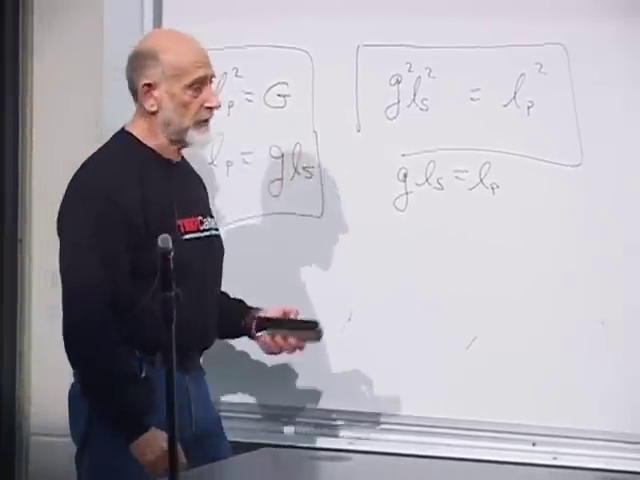
\includegraphics[width=0.72\textwidth]{lecture_06_figure_04.png}
\caption{黑板上保留的基本关系：\(\ell_p^2=G_N\)和\(\ell_p\sim g_s\ell_s\)。}
\lectureframe{00:15:45.000}
\end{figure}

方程~\eqref{eq:l06-newton-string}是本讲中始终使用的简化关系。\editorialnote{在紧致化的弦理论中，有效四维牛顿常数还依赖于紧致化体积和量级为一的约定。本讲将这些数据略去，以分离出对应关系的标度行为。}

\begin{classroomqa}
\audiencequestion{\(g_s\)大于还是小于一，哪个长度更大？\lecturetimestamp{00:16:00}}
\lecturerresponse{我们在弱耦合下工作，\(g_s<1\)。于是\(\ell_p\sim g_s\ell_s\)意味着弦长大于普朗克长度。强耦合需要不同的描述，此处不需要。}
\end{classroomqa}

\section{黑洞计数}

略去玻尔兹曼常数和数值因子，贝肯斯坦--霍金熵为
\begin{equation}
S_{\mathrm{BH}}=\frac{A}{4G_N}sim\frac{A}{G_N}sim\frac{A}{\ell_p^2}.
\label{eq:l06-bh-area}
\end{equation}
因子\(1/4\)在半经典公式中是精确的，但在这一标度论证中不起作用。

\begin{classroomqa}
\audiencequestion{下标``BH''是指黑洞还是贝肯斯坦--霍金？\lecturetimestamp{00:16:51}}
\lecturerresponse{就我们的目的而言，它可以同时提醒我们两者。重要的陈述是：熵是以普朗克面积度量的视界面积。}
\end{classroomqa}

对于四维施瓦茨席尔德黑洞，
\begin{equation}
R_s=2G_NM,
\qquad
A=4\pi R_s^2.
\end{equation}
如本讲所做的那样略去\(2\)和\(4\pi\)，
\begin{align}
S_{\mathrm{BH}}
&\sim \frac{R_s^2}{G_N}
\sim \frac{(G_NM)^2}{G_N} \\
&\sim M^2G_N
\sim M^2\ell_p^2.
\label{eq:l06-bh-mass}
\end{align}
这就是我们将与弦计数相比较的形式。

\section{长弦作为随机游走}

从一根小弦开始，向其中注入能量。一般的高激发弦不会保持为整齐的圈。它变成一个长而缠结的物体，就像卷线器严重缠乱后的钓鱼线。这一缠结具有熵，因为大量构型在宏观上看起来相同。

为了对它们计数，将空间替换为链路长度为\(\ell_s\)的点阵。格点是顶点，链路是线，基本方格是面。弦由连通的链路序列表示。这个模型是刻意粗糙的，但其指数式的态计数捕捉到了所需的标度行为。

\begin{figure}[htbp]
\centering
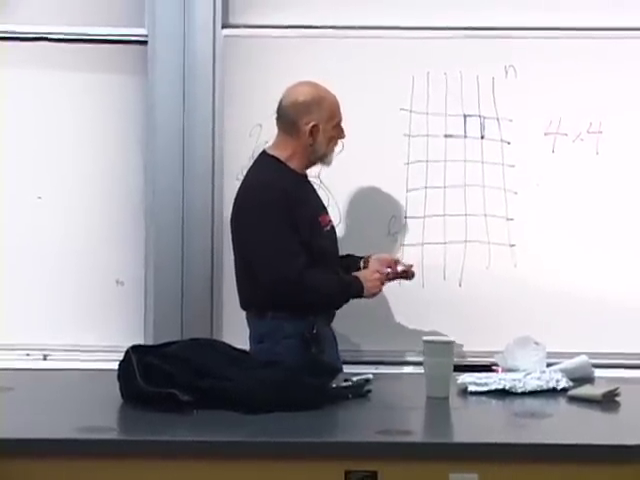
\includegraphics[width=0.72\textwidth]{lecture_06_figure_05.png}
\caption{二维点阵模型。蓝色线段标记弦的一步；在每个格点处对四种可能的延续进行计数。}
\lectureframe{00:23:50.000}
\end{figure}

\begin{classroomqa}
\audiencequestion{在这个玩具游走的每一步有多少种选择？\lecturetimestamp{00:22:43}}
\lecturerresponse{在正方点阵上是四种，因为允许立即回退。在三维中会有六种。换一种点阵会改变这个普通数字，但不会改变游走数目随链路数指数增长这一事实。}
\end{classroomqa}

如果弦有\(n\)条链路，二维玩具计数为
\begin{equation}
\Omega_n\sim4^n.
\label{eq:l06-walk-count}
\end{equation}
存在一种例外的直线游走，但它只是\(4^n\)中的一个态。典型的游走反复折叠，占据一个缠结的球。对于大的\(n\)，几乎每一个随机生成的构型在定性上都与任何其他构型相同。

熵是宏观上不可区分构型数目的对数：
\begin{equation}
S_{\mathrm{st}}=\log\Omega_n\sim n\log4\sim n.
\label{eq:l06-string-entropy-n}
\end{equation}

\begin{classroomqa}
\audiencequestion{为什么熵变得正比于\(n\)而不是\(4^n\)？\lecturetimestamp{00:25:39}}
\lecturerresponse{熵是态数目的对数。因此\(\log(4^n)=n\log4\)，而因子\(\log4\)是量级为一的常数，我们将把它略去。}
\end{classroomqa}

如果\(L\)是从弦的一端沿弦到另一端所得到的轮廓长度，那么
\begin{equation}
n=\frac{L}{\ell_s},
\qquad
S_{\mathrm{st}}\sim\frac{L}{\ell_s}.
\label{eq:l06-string-entropy-length}
\end{equation}
这里\(L\)不是缠结球的直径。它是沿弦测量的长得多的距离。

接下来我们用轮廓长度换取质量。在\(c=\hbar=1\)下，质量具有长度的倒数的量纲。因此一条弦尺度大小的链路携带量级为
\begin{equation}
m_{\mathrm{link}}\sim\frac{1}{\ell_s}.
\label{eq:l06-link-mass}
\end{equation}的质量

\begin{classroomqa}
\audiencequestion{为什么一条链路的质量必须按\(1/\ell_s\)标度？\lecturetimestamp{00:29:20}}
\lecturerresponse{在这些单位下，质量是长度的倒数，而\(\ell_s\)是唯一可用的长度。等价地，量级为\(1/\ell_s^2\)的弦张力乘以链路长度\(\ell_s\)给出相同的结果。}
\end{classroomqa}

于是完整弦具有
\begin{equation}
M\sim n m_{\mathrm{link}}
\sim\frac{n}{\ell_s}
\sim\frac{L}{\ell_s^2},
\qquad
L\sim M\ell_s^2.
\label{eq:l06-string-mass}
\end{equation}
将其代入方程~\eqref{eq:l06-string-entropy-length}得到
\begin{equation}
S_{\mathrm{st}}\sim M\ell_s.
\label{eq:l06-string-entropy-mass}
\end{equation}
点阵行走忽略了世界面约束和数值系数，但高度激发弦谱的指数增长给出了相同的领头标度行为。\editorialnote{随机行走构造是弦态高能级密度的一个助记手段，而不是对基本弦的字面离散化。}

\section{引发论证的不匹配}

现在两个答案为
\begin{equation}
S_{\mathrm{BH}}\sim M^2\ell_p^2,
\qquad
S_{\mathrm{st}}\sim M\ell_s.
\label{eq:l06-two-entropies}
\end{equation}
它们彼此相似，但在固定质量和任意耦合下并不相等。黑洞表达式对\(M\)是二次的；弦表达式则是线性的。不能简单地宣称热弦就是黑洞，而不解释这两个区域如何衔接。

\begin{figure}[htbp]
\centering
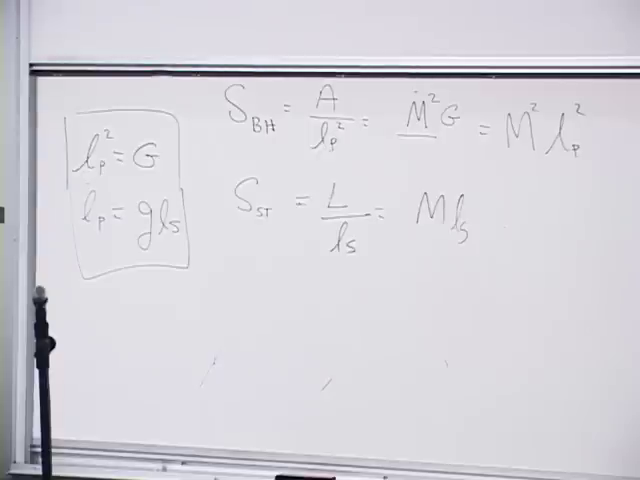
\includegraphics[width=0.78\textwidth]{lecture_06_figure_06.png}
\caption{无遮挡的板书对比：上方为黑洞熵，下方为长弦熵，左侧保留普朗克--弦关系。}
\lectureframe{00:33:20.000}
\end{figure}

课堂正是在这里暂停了。这种悬念是有用的：不匹配并非这一思想的失败，而是提示我们必须比较同一个态，同时改变引力的强度。

\section{转动耦合旋钮}

保持\(\ell_s\)固定，设想\(g_s\)可以变化。在\(g_s=0\)处，弦既不分裂也不结合，引力消失，因为\(G_N\sim g_s^2\ell_s^2\)。此时一个能量足够高的态就是一根长而弱相互作用的弦。

缓慢增大\(g_s\)。弦相互作用成为可能，而更重要的是，就当前论证而言，引力增强了。

\begin{classroomqa}
\audiencequestion{随着\(g_s\)增大，第一个效应是否仅仅是弦分裂成更短的弦？\lecturetimestamp{00:36:29}}
\lecturerresponse{分裂与结合成为可能，但保持\(\ell_s\)固定并追踪高熵态。核心效应是\(G_N\)增大，因此长弦的自引力将纠缠的球向内拉。}
\end{classroomqa}

该物体收缩并变得更致密。其引力势能为负，因此收缩降低其总能量，从而降低其质量。

\begin{classroomqa}
\audiencequestion{当自引力将弦拉在一起时，能量是增加还是减少？\lecturetimestamp{00:37:48}}
\lecturerresponse{它减少。结合能变得更负。尽管我们继续追踪同一个态，沿路径的质量不必保持不变。}
\end{classroomqa}

最终该物体的尺度与其施瓦西半径相当。超过这一点，黑洞描述就是自然的描述。更大的初始激发在更小的耦合下达到这一条件，因为更 massive 的物体形成视界所需的引力强度更小。

\begin{figure}[htbp]
\centering
\resizebox{0.95\linewidth}{!}{%
\begin{tikzpicture}[x=1cm,y=1cm,>=Latex]
  \draw[->,line width=0.9pt] (0,0) -- (11,0) node[right] {increasing \(g_s\)};
  \node[draw,rounded corners,align=center,minimum width=2.6cm,minimum height=1.15cm] at (1.8,1.5) {long excited string\\weak self-gravity};
  \node[draw,rounded corners,align=center,minimum width=2.6cm,minimum height=1.15cm] at (5.5,1.5) {correspondence point\\\(R_s\sim\ell_s\)};
  \node[draw,circle,align=center,minimum size=1.8cm] at (9.3,1.5) {black\\hole};
  \draw[->,line width=0.8pt] (3.15,1.5) -- (4.1,1.5) node[midway,above,font=\small] {contracts};
  \draw[->,line width=0.8pt] (6.9,1.5) -- (8.25,1.5);
  \node[font=\small,align=center] at (5.5,-0.65) {same family of states followed slowly;\\binding energy and mass may change};
\end{tikzpicture}
}
\caption{固定\(\ell_s\)下的对应路径。反转箭头将黑洞态带回长弦态。}
\end{figure}

\begin{classroomqa}
\audiencequestion{我们是否应设想\(g_s\)介于零和一之间？\lecturetimestamp{00:40:18}}
\lecturerresponse{是的。论证仍处于弱耦合区域。如果\(g_s\)非常小，则该态必须相应地非常 massive 才能成为黑洞。我们不需要进入控制很差的\(g_s>1\)区域。}
\end{classroomqa}

在思想实验中，缓慢的变化是可逆的。

\begin{classroomqa}
\audiencequestion{如果我们把耦合调回去，直到引力不再能把黑洞束缚在一起，它会变成什么？\lecturetimestamp{00:41:37}}
\lecturerresponse{一根长弦。在引力消失时，这一构造中的一切都必须用弦态来描述。朝一个方向转动旋钮将弦映射为黑洞；转回来则将黑洞映射为弦。}
\end{classroomqa}

在固定总能量和固定体积内，占主导的高熵构型本质上是一根长弦，而不是数量巨大的短弦。这一陈述在此并未推导。它是弦在Hagedorn区域附近的统计力学结果，之后会重新讨论。

\section{外部观察者看到什么}

当该物体被描述为黑洞时，弦在哪里？在外部描述中，它并不会突然消失。施瓦西时间将表观穿越送到任意晚的时间，因此弦的自由度被表示为在视界上或视界附近积累。

\begin{figure}[htbp]
\centering
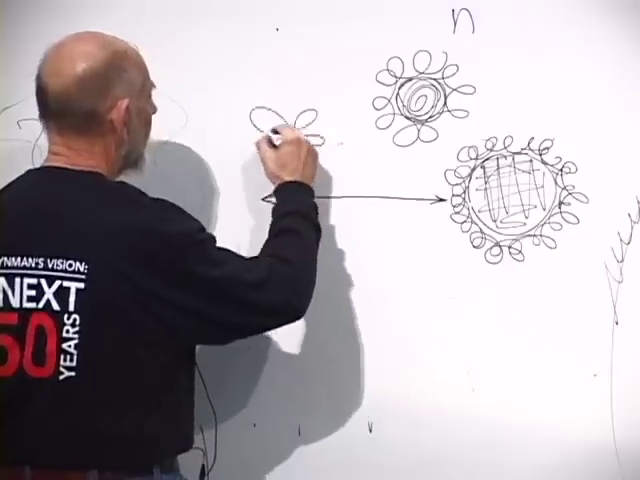
\includegraphics[width=0.72\textwidth]{lecture_06_figure_07.png}
\caption{板书对比：宏观视界中弦尺度结构只是薄薄的绒毛，而较小视界的半径接近圈尺度。}
\lectureframe{00:45:30.000}
\end{figure}

对于\(R_s\gg\ell_s\)，黑洞是宏观的，弦尺度结构相对于视界半径而言只是一层薄薄的壳层。当半径减小到接近\(\ell_s\)时，光滑黑洞与延展弦之间的区分就失去了意义。这是一种外部的、拉伸视界描述；不应将其与一种坐标无关的断言相混淆，即下落物质永远不会穿过一个规则视界。\editorialnote{讲座使用的是黑洞互补性中为人熟知的外部描述。短语``在视界上''指的是由外部描述所分辨的自由度，而不是对其协变位置的独立推导。}

交叉发生在
\begin{equation}
R_s\sim\ell_s.
\label{eq:l06-correspondence-radius}
\end{equation}
低于弦尺度时，施瓦茨席尔德几何无法分辨本应支撑它的结构。圈从本应是视界的位置涨落开去，该态更适合被称为弦。

\section{对应点}

在方程~\eqref{eq:l06-correspondence-radius}中使用\(R_s\sim G_NM\)：
\begin{equation}
G_NM\sim\ell_s.
\end{equation}
然后代入\(G_N\sim g_s^2\ell_s^2\)：
\begin{equation}
M g_s^2\ell_s^2\sim\ell_s,
\qquad
M g_s^2\ell_s\sim1.
\label{eq:l06-correspondence-condition}
\end{equation}

\begin{figure}[htbp]
\centering
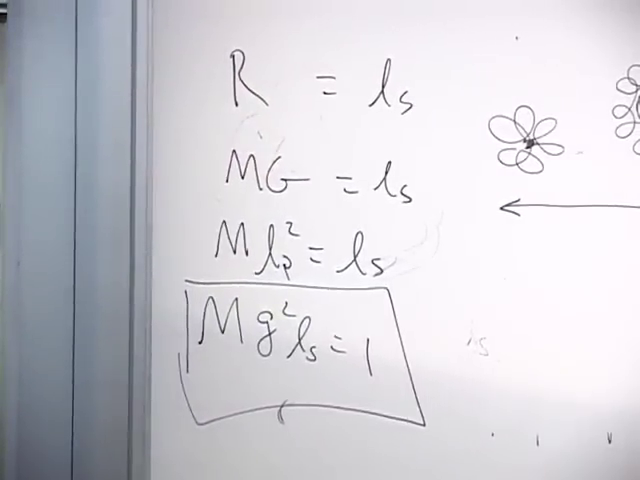
\includegraphics[width=0.72\textwidth]{lecture_06_figure_08.png}
\caption{黑板上完成的过渡代数：\(R_s\sim\ell_s\)导致加框的无量纲条件\(Mg_s^2\ell_s\sim1\)。}
\lectureframe{00:49:50.000}
\end{figure}

一位听众注意到了这个条件正在准备什么。在对应点，
\begin{align}
S_{\mathrm{BH}}
&\sim M^2\ell_p^2
\sim M^2g_s^2\ell_s^2 \\
&=(M\ell_s)(Mg_s^2\ell_s)
\sim M\ell_s
\sim S_{\mathrm{st}}.
\label{eq:l06-entropy-preview}
\end{align}

\begin{classroomqa}
\audiencequestion{这些方程是否已经意味着黑洞熵与弦熵变得相等？\lecturetimestamp{00:50:18}}
\lecturerresponse{是的。这正是计算所要达到的地方。各个要素已经放在黑板上，但讲座推迟了它们的完整组装，以便能够仔细审视对应的逻辑。}
\end{classroomqa}

方程~\eqref{eq:l06-entropy-preview}是这次交流中隐含的一行代数预览。它确立了标度关系，而不是精确系数\(1/4\)。精确的微观匹配需要更受控的黑洞和更详细的弦构造。\editorialnote{讲座在将方程~\eqref{eq:l06-entropy-preview}作为其完整推导呈现之前就停止了。这里将其写出，是因为听众明确指出了这一等式，而且所有所需的关系都已经出现过。}

\section{为什么熵可以被携带过去}

还剩下一个逻辑要素。假设一个控制参数，例如磁场或\(g_s\)，在系统孤立且演化可逆的情况下被足够缓慢地改变。能量、大小和结合能可能改变，但熵保持不变：
\begin{equation}
\Delta S=0.
\label{eq:l06-adiabatic-entropy}
\end{equation}
讲座将此与信息守恒联系起来。熵衡量的是被粗粒化描述所隐藏的信息；哈密顿量的缓慢可逆变化重新排列了态，而没有删除该信息。

\begin{classroomqa}
\audiencequestion{熵恒定是否要求路径避开相变？\lecturetimestamp{00:54:01}}
\lecturerresponse{是的，必须能够连续地跟踪该态。有限系统没有无限体积那种严格非解析的热力学相变，而且如果变化足够缓慢，对应可以被视为光滑的交叉。}
\end{classroomqa}

这里使用的绝热是更强的准静态、可逆意义。绝热但不可逆的过程可以产生熵；缓慢性和跟踪态的能力是必不可少的。\editorialnote{热力学陈述\(\Delta S=0\)要求一条可逆绝热路径。在量子力学中，相应的想法是当参数变化时跟踪同一组态，而不发生不受控的能级跃迁。}

\begin{classroomqa}
\audiencequestion{为什么一根长弦会比携带相同总质量的几根较短弦具有更多熵？\lecturetimestamp{00:54:44}}
\lecturerresponse{这反直觉，但显式的高能态计数在固定体积中偏向长弦成分。证明被推迟；就目前的论证而言，我们只需要黑洞映射到最大熵的弦部门，而不是映射到由极多短弦组成的稀薄气体。}
\end{classroomqa}

因此操作策略是：
\begin{enumerate}
\item 从耦合\(g_{s,0}\)下质量为\(M_0\)的黑洞开始。
\item 缓慢降低\(g_s\)，同时跟踪同一高熵态族。
\item 停在\(R_s\sim\ell_s\)处，此时黑洞描述变为长弦描述。
\item 使用\(S_{\mathrm{st}}\sim M\ell_s\)计数弦态。
\item 将该熵沿可逆路径带回原来的黑洞。
\end{enumerate}

\begin{figure}[htbp]
\centering
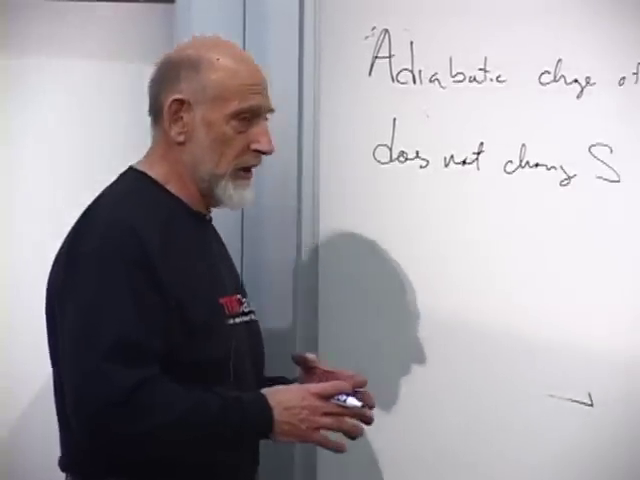
\includegraphics[width=0.72\textwidth]{lecture_06_figure_09.png}
\caption{在陈述策略时保留在黑板上的一条原理：\(g_s\)的绝热变化不改变\(S\)。}
\lectureframe{00:56:40.000}
\end{figure}

弦理论已经为带电、旋转、超对称、近极端以及高维黑洞给出了更为精确的熵计数。这里关于中性Schwarzschild黑洞的讨论是粗略的对应论证：它确定了态密度的参数依赖关系和物理交叉，而不是精确的受保护简并度。\editorialnote{精确一致对于态计数在耦合变化时受到保护的特殊黑洞最为有力。本讲有意给出最简单的量级版本。}

\begin{classroomqa}
\audiencequestion{当引力被关闭时，态是否可能变成两根弦，而不是恰好一根？\lecturetimestamp{00:58:25}}
\lecturerresponse{存在有限概率出现少量长弦，而使用两根而非一根不会改变主导的熵标度。会改变论证的是碎裂成大量短弦组成的气体；高能统计计数并不支持这一结果。}
\end{classroomqa}

黑洞是能够装入一个区域的最大熵，而长弦是引力被移除时相应的高熵态。这两种描述现在已被联系起来，但尚未发展成精确计算。下一步是仔细重复代数运算，并追问这一对应关系可以被信任到何种程度。
